%!TEX root = ../report.tex

%
% Introduction
%

\section{Introduction}
\label{sec:introduction}

% General description of the problem and its context, current 
% solutions, and road map of the project.
% 2 - 3 pages
% TODO: Mobile proximity based apps (Special kind of context aware), Explain context-aware, Examples
% Technologies to know if the user is nearby some POI
% Development of proximity-based apps
% Smart spaces
% TODO: What are native and web mobile apps
% TODO: What makes more sense to proximity-based apps
% (Native vs Web)
% This paper is about...
% Present next sections

% Problem
The use of context-aware mobile apps has been increasing.
Context-aware mobile apps are apps that use data, acquired
from one or more sensors and other user's data, 
such as the calendar. For instance, it is possible to
build an app that puts the phone, in silent mode, if the
user is in a meeting. Proximity-based apps are
context-aware apps that allow the user to interact
with the app if he is nearby some point of interest.
Table \ref{tab:statistics} shows some examples of proximity-based
apps and their number of installs and rating in Google
Play Store and Apple App Store. 

\begin{table}[h]
\centering
\begin{tabular}{|l|l|l|r|l}
\cline{1-4}
App & Store & Downloads & \multicolumn{1}{c|}{Rating (from 0 to 5)} &  \\ \cline{1-4}
Foursquare & Google Play Store & \num{10000000} - \num{50000000} & 4.1 &  \\ \cline{1-4}
Skout & Google Play Store & \num{10000000} - \num{50000000} & 4.1 &  \\ \cline{1-4}
Tinder & Google Play Store & \num{10000000} - \num{50000000} & 4.1 &  \\ \hline
\end{tabular}
\caption{Statistics about some existent proximity-based apps}
\label{tab:statistics}
\end{table}

%Compared wth most used.
% ratio proximity-based/most used installs
% ratings are almost the same

In table \ref{tab:most_used} there are some statistics about
some of the most popular apps. Facebook is the app with the
greatest number of downloads. One of the apps of table
\ref{tab:statistics} has, at least, \num{1e7} downloads.
Facebook has, at least, \num{1e9}. Twitter and Instagram
have, at least, \num{1e8} downloads. Which means, one of
the apps of table \ref{tab:statistics} represents
1/100 of Facebook's downloads and 1/10 of Twitter's
and Instagram's downloads. In terms of rating, the
values in table \ref{tab:statistics} are similar to table
\ref{tab:most_used}.

\begin{table}[h]
\centering
\begin{tabular}{|l|l|l|r|l}
\cline{1-4}
App & Store & Downloads & \multicolumn{1}{c|}{Rating (from 0 to 5)} &  \\ \cline{1-4}
Facebook & Google Play Store & \num{1e9} - \num{5e9} & 4.0 &  \\ \cline{1-4}
Twitter & Google Play Store & \num{1e8} - \num{5e8} & 4.1 &  \\ \cline{1-4}
Instagram & Google Play Store & \num{1e8} - \num{5e8} & 4.5 &  \\ \hline
\end{tabular}
\caption{Statistics about most-used apps}
\label{tab:most_used}
\end{table}



% Possible solutions
To know if the user is nearby some point of interest,
we need to know the user's location. We can use GPS to
get this information. Most apps use this technology because
most smartphones have a GPS receiver. 
%Show some statistics about smartphones with GPS
Unfortunately, GPS cannot be used indoors. The signal can
be very weak inside a building. To make proximity-based
apps work properly indoors, we need to use other 
technologies.
\subsection{Bluetooth Low Energy}
\label{sub:bluetooth_low_energy}
Bluetooth Low Energy (BLE) is a possibility 
and it is starting to be used for this kind of apps.
BLE Beacons are devices, that use BLE, to broadcast a 
universally unique identifier (UUID). A smartphone that
supports BLE can get this signal. But, only smartphones
with Bluetooth, at least, version 4, support BLE.
For instance, a store owner wants to advertise a promotion
to potential customers that are nearby his store. To 
achieve this goal, the store owner would need to put
a beacon inside his store and his customers would need an
app that would get the beacon's signal and show a 
notification in the customers' smartphones,
as it is shown figure \ref{fig:store_example}.
\begin{figure}[!ht]
  \centering
    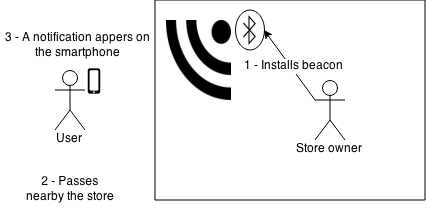
\includegraphics[width=0.9\textwidth]{img/store_example}
    \caption{Interaction between the user's smartphone
    and a beacon inside a store}
    \label{fig:store_example}
\end{figure}

To develop these apps, that use beacons, we can use the 
BLE API that each 
mobile platform provides or simply the Software
Development Kit (SDK) from the 
beacons vendor. The example of the store owner is a
simple one. The app just gets the signal and show a 
notification. However, if the store owner has more than
one store and wants to show a different promotion depending
on each store, the app would need to do more than just get
the beacon's signal. After getting the signal, the app
would get the promotion for that beacon, from a 
back-end. The developer of this app, would need to
write the code that gets the beacon's signal and also
the code that will get the information from the back-end.

Another example could be an app for a museum. The owner
of a museum wants to show more information, in the 
visitors' smartphones, about the pieces that are in a given
room. He would need one beacon for each piece and an app
that would get the beacon's signal and use a
back-end to get the right information about a given piece.
The museum needs to advertise, to its visitors, that such
an app exists and also, tell them to download the app
before they enter the museum. The developers of the
store and the museum apps will write similar code to get
the beacon's signal and get data from a back-end.

\subsection{Smart Places}
\label{sub:smart_places}
Before going further, we will introduce the concept of
smart place. Smart places are places that can, somehow,
interact with users nearby and users can interact 
with them.
In this context, a smart place have beacons and the users
have apps, installed in their smartphones, that can interact
with them and show relevant information to the user.
With this definition, we can say, about the examples above,
that the owners of the store and the museum, want to
turn their places into smart places.
If there is another smart place, the user would need to
install another app.
Any mobile app can be a native or a web app. Native apps
are apps that we have to install and that can access
device's features, such as BLE. Web apps are web
applications, designed for mobile devices, that run
on the device's browser. This apps do not need to be
installed but they do not have access
to same device's features that native apps have.
Mobile apps for smart spaces, according to our definition,
need to be native, because we need to get signals from
nearby beacons. For that, we need to use bluetooth, which is
not available in web apps, since they run in the browser.
We would like to have the best of both sides. In one side,
native apps can detect nearby beacons. In the other side,
web apps do not need to be installed.

We propose a framework, to develop mobile web apps for smart
places, that allow developers to only write the code
for the application logic and the specific behavior when
the user is nearby specific points of interest (POI).
Each beacon represents one POI. Developers would not need
to write the code that gets beacons' data and get the
right information from a back-end. They would need only
to write the code for each specific POI. They could give
a name to each POI and the app will receive that name 
instead of the beacon's raw data. 

Since mobile web
apps do not need to be installed, we choose to support
them instead of native, to allow
the user to have access to any app in any smart place.
This apps run on the device's browser. However, detecting
nearby beacons is not a feature integrated in the mobile
Operating System. Our solution would be to build the
Smart Places App,
that detects nearby beacons, turn them into names and
other high-level information, and deliver it to the
mobile web app. The user would need only this app to
be able to access any smart place app. Also, the same app
could be used to configure a smart place.
For instance, a restaurant's owner wants to offer, to
his customers, the possibility to make their orders,
as soon as they sit, from their smartphones. Some
developers, could develop the app for restaurants,
using our framework. This developers would only think
about tables instead of beacons. The owner would need
to put a beacon in each table. After the beacons
installation, he could just use the Smart Places App,
choose the app for restaurants, and put his smartphone
closer to a beacon and configure it. This configuration
would be, for each beacon, what is the number of the table
where it is deployed. Then, his customers would only
need the Smart Places App, turn on bluetooth and they will
be notified that they can make their orders from their
smartphones.

In next section \ref{sec:objectives}, we describe the main
objectives of the project proposed here.
Section \ref{sec:related_work} describes related
work about the development and deployment of
context aware mobile apps.
In \ref{sec:architecture} it is explained the architecture of our solution. The main components and the role of
each one.
Section \ref{sec:evaluation} is about how we are going
to evaluate our solution.
Finally, last section \ref{sec:conclusions} we conclude
the paper.
